\chapter{Dados de Perfilagem}

As RNAs são capazes de reconhecer padrões \citep{Konate2014,Kumar2015}. E padrões muitas vezes são recorrentes no tocante a geologia \citep{Vail_1977}. 

Ciclos de deposição de siltes e argilas e areias muitas vezes são controlados pelas variações constantes das estações do ano \citep{Milani1998,CristinaLopesQuintas1999,Milani2000} . Esse registro litológico se faz presente em dados de poços em todo o mundo \citep{Scherer2006}.

Em uma perfilagem de poço composta são realizadas diversas medidas de propriedades físicas que ao serem analisadas, em conjunto, tornam possível ao geólogo identificar mudanças litológicas e consequentemente topos e bases de camadas de interesse \citep{FrancaAlmerio&Potter1991,Zalan2007,artur_paleoestruturas_2008}. 

A Fig. \ref{PerfilComposto} ilustra a disposição de um perfil de poço associado com topos e bases de rochas. 

\begin{figure}[H]
		\centering
	\setlength{\fboxsep}{8pt}
	\setlength{\fboxrule}{0.1pt}
	\fbox{
	\includegraphics[scale=0.16]{Imagens/poco.png}
}
	\caption{Exemplo de um dado público de uma perfilagem de poço composta realizada pela Petrobras, na Bacia do Paraná.}
	\label{PerfilComposto}
\end{figure}

Entretanto não é toda a perfilagem de poço que contém o topo e base de camada. As RNAs se apresentam como uma solução para o problema de identificação litológica e dos topos e bases dessas camadas. Uma vez observado que a variação das propriedades físicas das rochas em subsuperfície variam obedecendo certos padrões \citep{Yan2014}. 

Em \citet{Telford_1993}, encontram-se variações das propriedades físicas dos principais grupos de rochas. A Tab. \ref{rock-properties1} e a Tab. \ref{rock-properties2} apresentam um compêndio desses principais valores.  

\begin{table}[H]
	\centering
	\caption{Compilação de Perfis usados na inferência de litologia.}
	\label{rock-properties1}
	\begin{tabular}{@{}llllllllll@{}}
		\toprule
		Rocha         & Densidade ($g/cm^{3}$) & Raios-Gama ($Ci/g$)& Potencial-Espontâneo ($mV$)&   \\ \midrule
		Conglomerado &     $2,50$  &       ---        &    ---        &      \\
		Arenito  &    $2,35$      &       $2,00\leftrightarrow4,00$       &     ---       &      \\
		Folhelho &   $2,40$       &      ---        &      ---      &    \\
		Argilito &     $2,55$   &          ---     &       ---     &     \\
		Siltito  &      $2,21$    &          ---     &       ---     &   \\
		Dolomita &     $2,70$    &        $8,00$       &   ---         &       \\
		Marga  &    $2,50$     &         ---      &    ---        &     \\
		Basalto  &     $2,99$    &          $0,50$     &    ---       &      \\
		Diabásio &    $2,90$    &         ---      &       ---     &     \\
		Lava &     $2,61$    &      $0,33$         &      ---      &      \\
		Granito &    $2,64$      &       $0,70\leftrightarrow4,80$        &      ---      &      \\
		Gabro &    $3,03$     &       ---        &     ---       &       \\
		Peridotito &   $3,15$    &      ---         &     ---       &      \\
		Quartzito &    $2,60$    &        $5,00$      &     ---       &    \\
		Xisto &   $2,64$    &         ---      &      ---      &    \\
		Gnaisse &    $2,80$     &      ---         &    ---        &        \\
		Serpentinito &    $2,78$     &   ---            &   ---     &        \\
		Anfibolito &  $2,96$       &          ---     &       ---     &        \\
		Eclogito &  $3,37$    &       ---        &      ---      &    \\
		Mármore &   $2,75$       &      ---         &     ---       &      \\ \bottomrule
	\end{tabular}
\end{table}

\begin{table}[H]
	\centering
	\caption{Compilação de Perfis usados na inferência de porosidade, permeabilidade.}
	\label{rock-properties2}
	\begin{tabular}{@{}llllllllll@{}}
		\toprule
		Rocha   & Resistividade ($\Omega/m$) &  Neutrão ($API$) & Velocidade ($km/s$)  &    \\ \midrule
		Conglomerado &    $2\times10^{3}\leftrightarrow10^{4}$       &    ---           &     $1,80\leftrightarrow4,90$       &     \\
		Arenito  &    $1\leftrightarrow6,4\times10^{8}$       &      ---         &     $4,00\leftrightarrow4,30$       &   \\
		Folhelho &     $50\leftrightarrow10^{7}$      &      ---         &      $2,15\leftrightarrow3,30$      &   \\
		Argilito &     $10\leftrightarrow8\times10^{2}$      &       ---        &     ---       &      \\
		Siltito  &      $1\leftrightarrow100$     &      ---         &         $4,00\leftrightarrow6,20$    &         \\
		Dolomita &   $3,5\times10^{2}\leftrightarrow5\times10^{3}$        &    ---           &      $5,70\leftrightarrow6,00$      &      \\
		Marga  &     $3\leftrightarrow70$      &     ---          &     ---       &     \\
		Basalto  &     $10\leftrightarrow1,3\times10^{7}$      &     ---          &     $ 5,00\leftrightarrow5.80$         &     \\
		Diabásio &  $20\leftrightarrow5\times10^{7}$         &      ---         &     ---       &  \\
		Granito Porfirítico (seco) &     $1,3\times10^{6}$     &       ---        &     $5,80$       &    \\
		Granito Porfirítico (úmido) &  $4,5\times10^{3}$          &      ---         &     $ 5,00\leftrightarrow5.60$         &      \\
		Gabro &   $10^{3}\leftrightarrow10^{6}$       &      ---         &      $ 5,00\leftrightarrow5.80$        &     \\
		Peridotito (seco) &   $6,5\times10^{3}$        &    ---           &       ---     &    \\
		Peridotito (úmido) &    $3\times10^{3}$       &      ---         &      ---      &  \\
		Xisto &    $20\leftrightarrow10^{4}$       &        ---       &       ---     &   \\
		Gnaisse (seco) & $3\times10^{6}$          &         ---      &     ---       &   \\
		Gnaisse (úmido) &   $6,8\times10^{4}$        &       ---        &      ---      &   \\
		Tufa (seca) &      $2\times10^{3}$     &      ---         &     $1,80\leftrightarrow3,50$       &     \\
		Tufa (úmida) &     $10^{5}$      &     ---          &     ---       &      \\
		Mármore &  $10^{2}\leftrightarrow2,5\times10^{8}$         &       ---        &      ---      &    \\ \bottomrule
	\end{tabular}
\end{table}

%FALAR DO TRATAMENTO DO DADO, DO NEURÔNIO, DA GEOMETRIA DA REDE, DO TREINO, DA FUNÇÃO DE ATIVAÇÃO, CAMADAS OCULTAS, PESOS.%
 

\section{Modelo proposto para gerar os dados sintéticos}

O modelo proposto para o teste da rede neuronal foi concebido com base em um modelo geológico esquemático proposto por  \citet{Sal2008} \textit{apud} \citep{Eiras1996}. Esta simplificação reproduz, em uma bacia do tipo sinéclise, estruturas geológicas como Horts, Grábens, semi-grábens, falhas normais, reversas. E representa ainda processos halocinéticos referenciados por \cite{Eiras1996}.

A Fig. \ref{modelo} representa o modelo em tratado anteriormente. A caixa aumentativa evidencia a falha normal, representada no dado de poço por um contato não plano-paralelo.

\begin{figure}[H]
	\centering
	\setlength{\fboxsep}{8pt}
	\setlength{\fboxrule}{0.1pt}
	\fbox{
		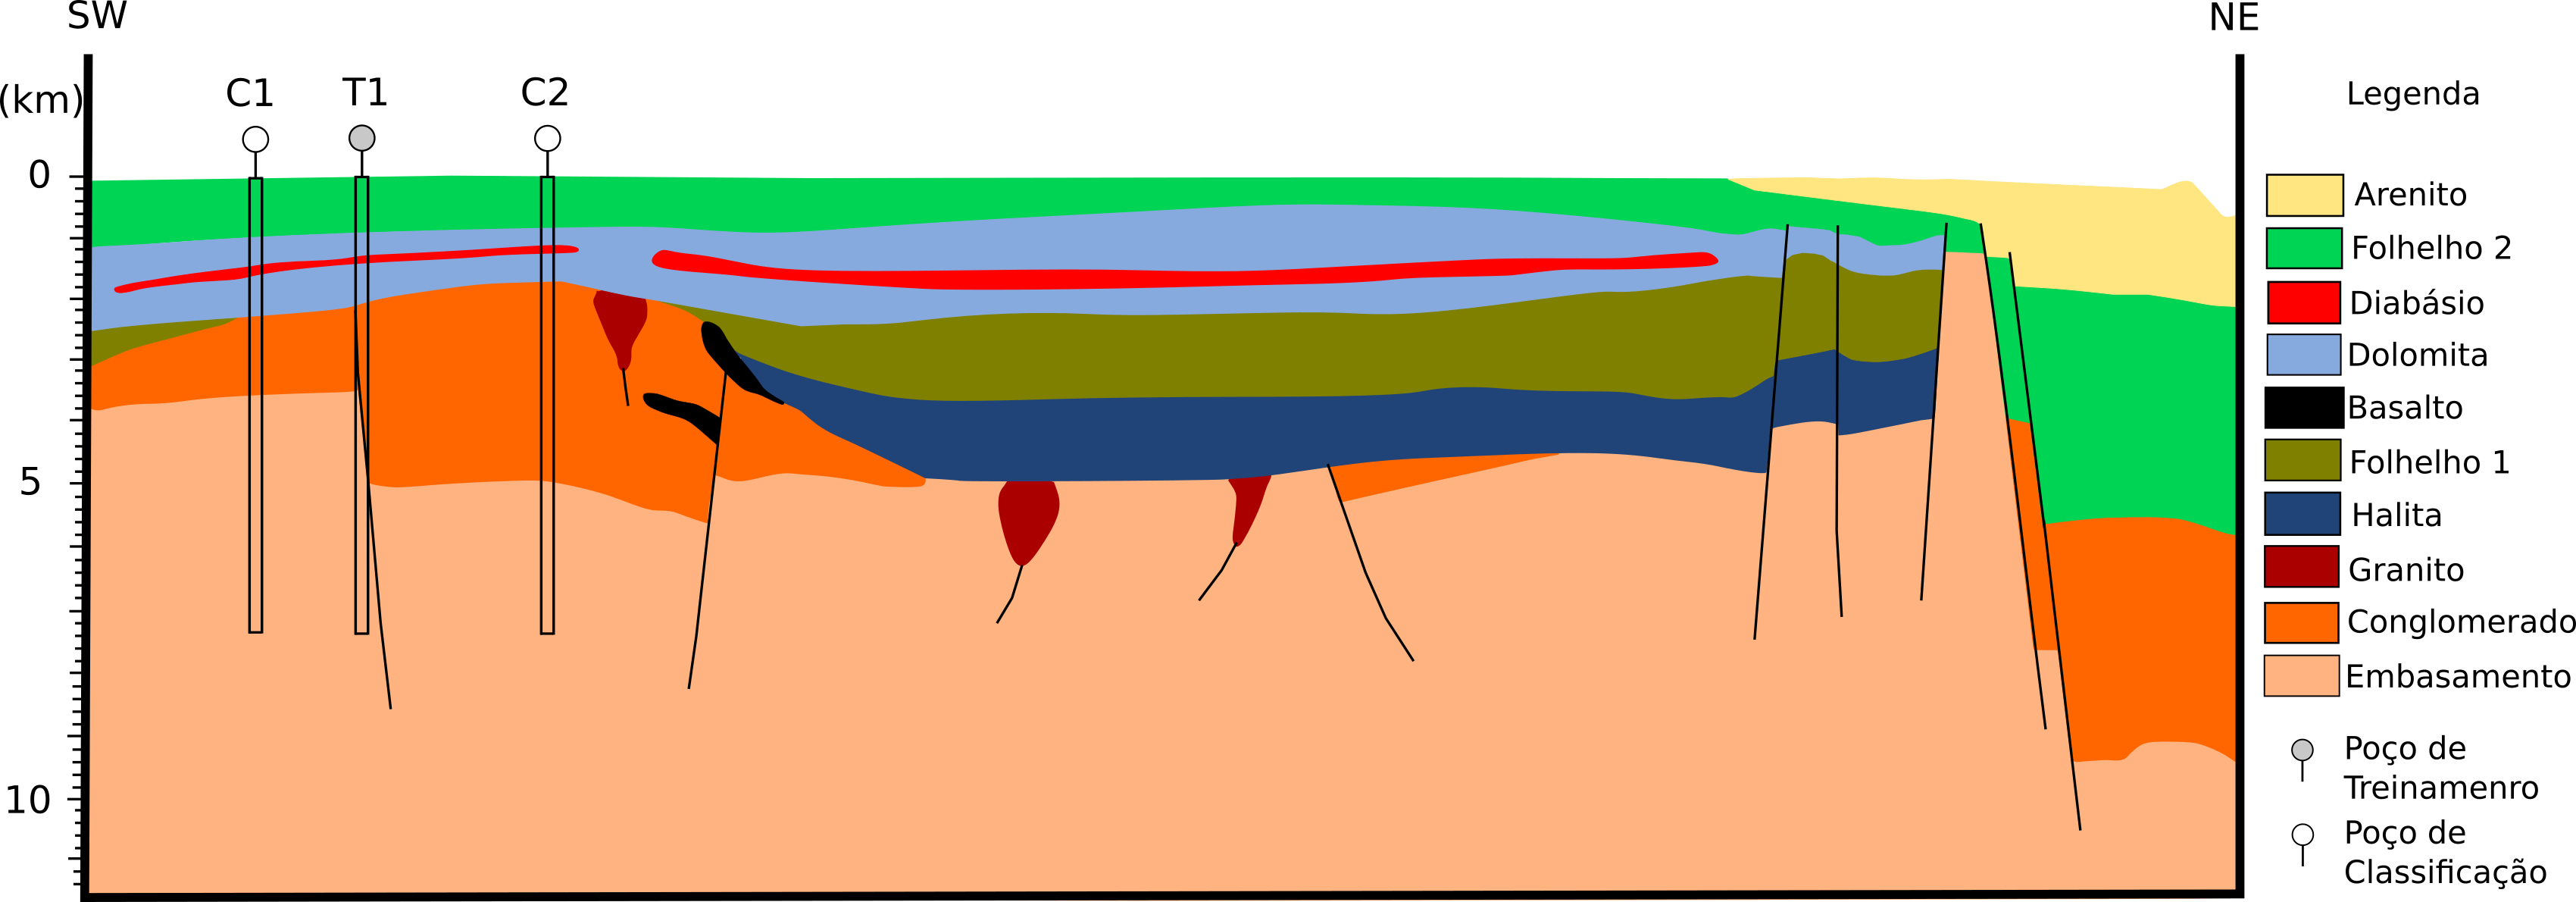
\includegraphics[scale=0.5]{Imagens/Modelo.png}
	}
	\caption{Modelo Simplificado baseado em \cite{Sal2008}.}
	\label{modelo}
\end{figure}

A partir da Fig. \ref{modelo} foram gerados três poços, na parte SW do perfil, com profundidades de $7$ km cada. Os três poços contém um conjunto com $4$ dados de propriedades físicas que são densidade, raio-gama, resistividade e velocidade, respectivamente. Os valores de propriedades físicas utilizados foram  baseados, em resultados já publicados, na literatura geocientífica, anteriormente, e retirados de \citet{Telford_1993}. Os poços simulam dados de \textit{well logging} com uma taxa de amostragem de $10$ m.

Os poços simulam diferentes padrões interpretativos usuais da ciência de perfilagem \footnote{Padrões usuais reconhecido por intérpretes geralmente associados a horizontes de interesse. Esses padrões são identificados como padrões sinos, sinos invertidos, serra e caixa.}. O poço denominado T$1$ \footnote{T$1$: poço escolhido para treinar a rede neuronal.} se localiza entre os poços C$1$ e C$2$ atravessando uma falha normal. 

A Fig. \ref{T1} apresenta os dados do poço T1. As espessuras das camadas são de $800$ m de embasamento, $2$ km de uma mistura crescente entre conglomerado e embasamento, perfazendo um padrão sino nos dados de perfilagem, $2$ km de conglomerado, $1$ km de dolomita (pacote inferior), $300$ m de diabásio, $400$ m de dolomita (pacote superior), $600$ m de folhelho $2$. A falha foi representada por uma função linear da variação de profundidade por propriedade física de uma mistura crescente de conglomerado e embasamento.

\begin{figure}[H]
	\centering
	\setlength{\fboxsep}{8pt}
	\setlength{\fboxrule}{0.1pt}
	\fbox{
		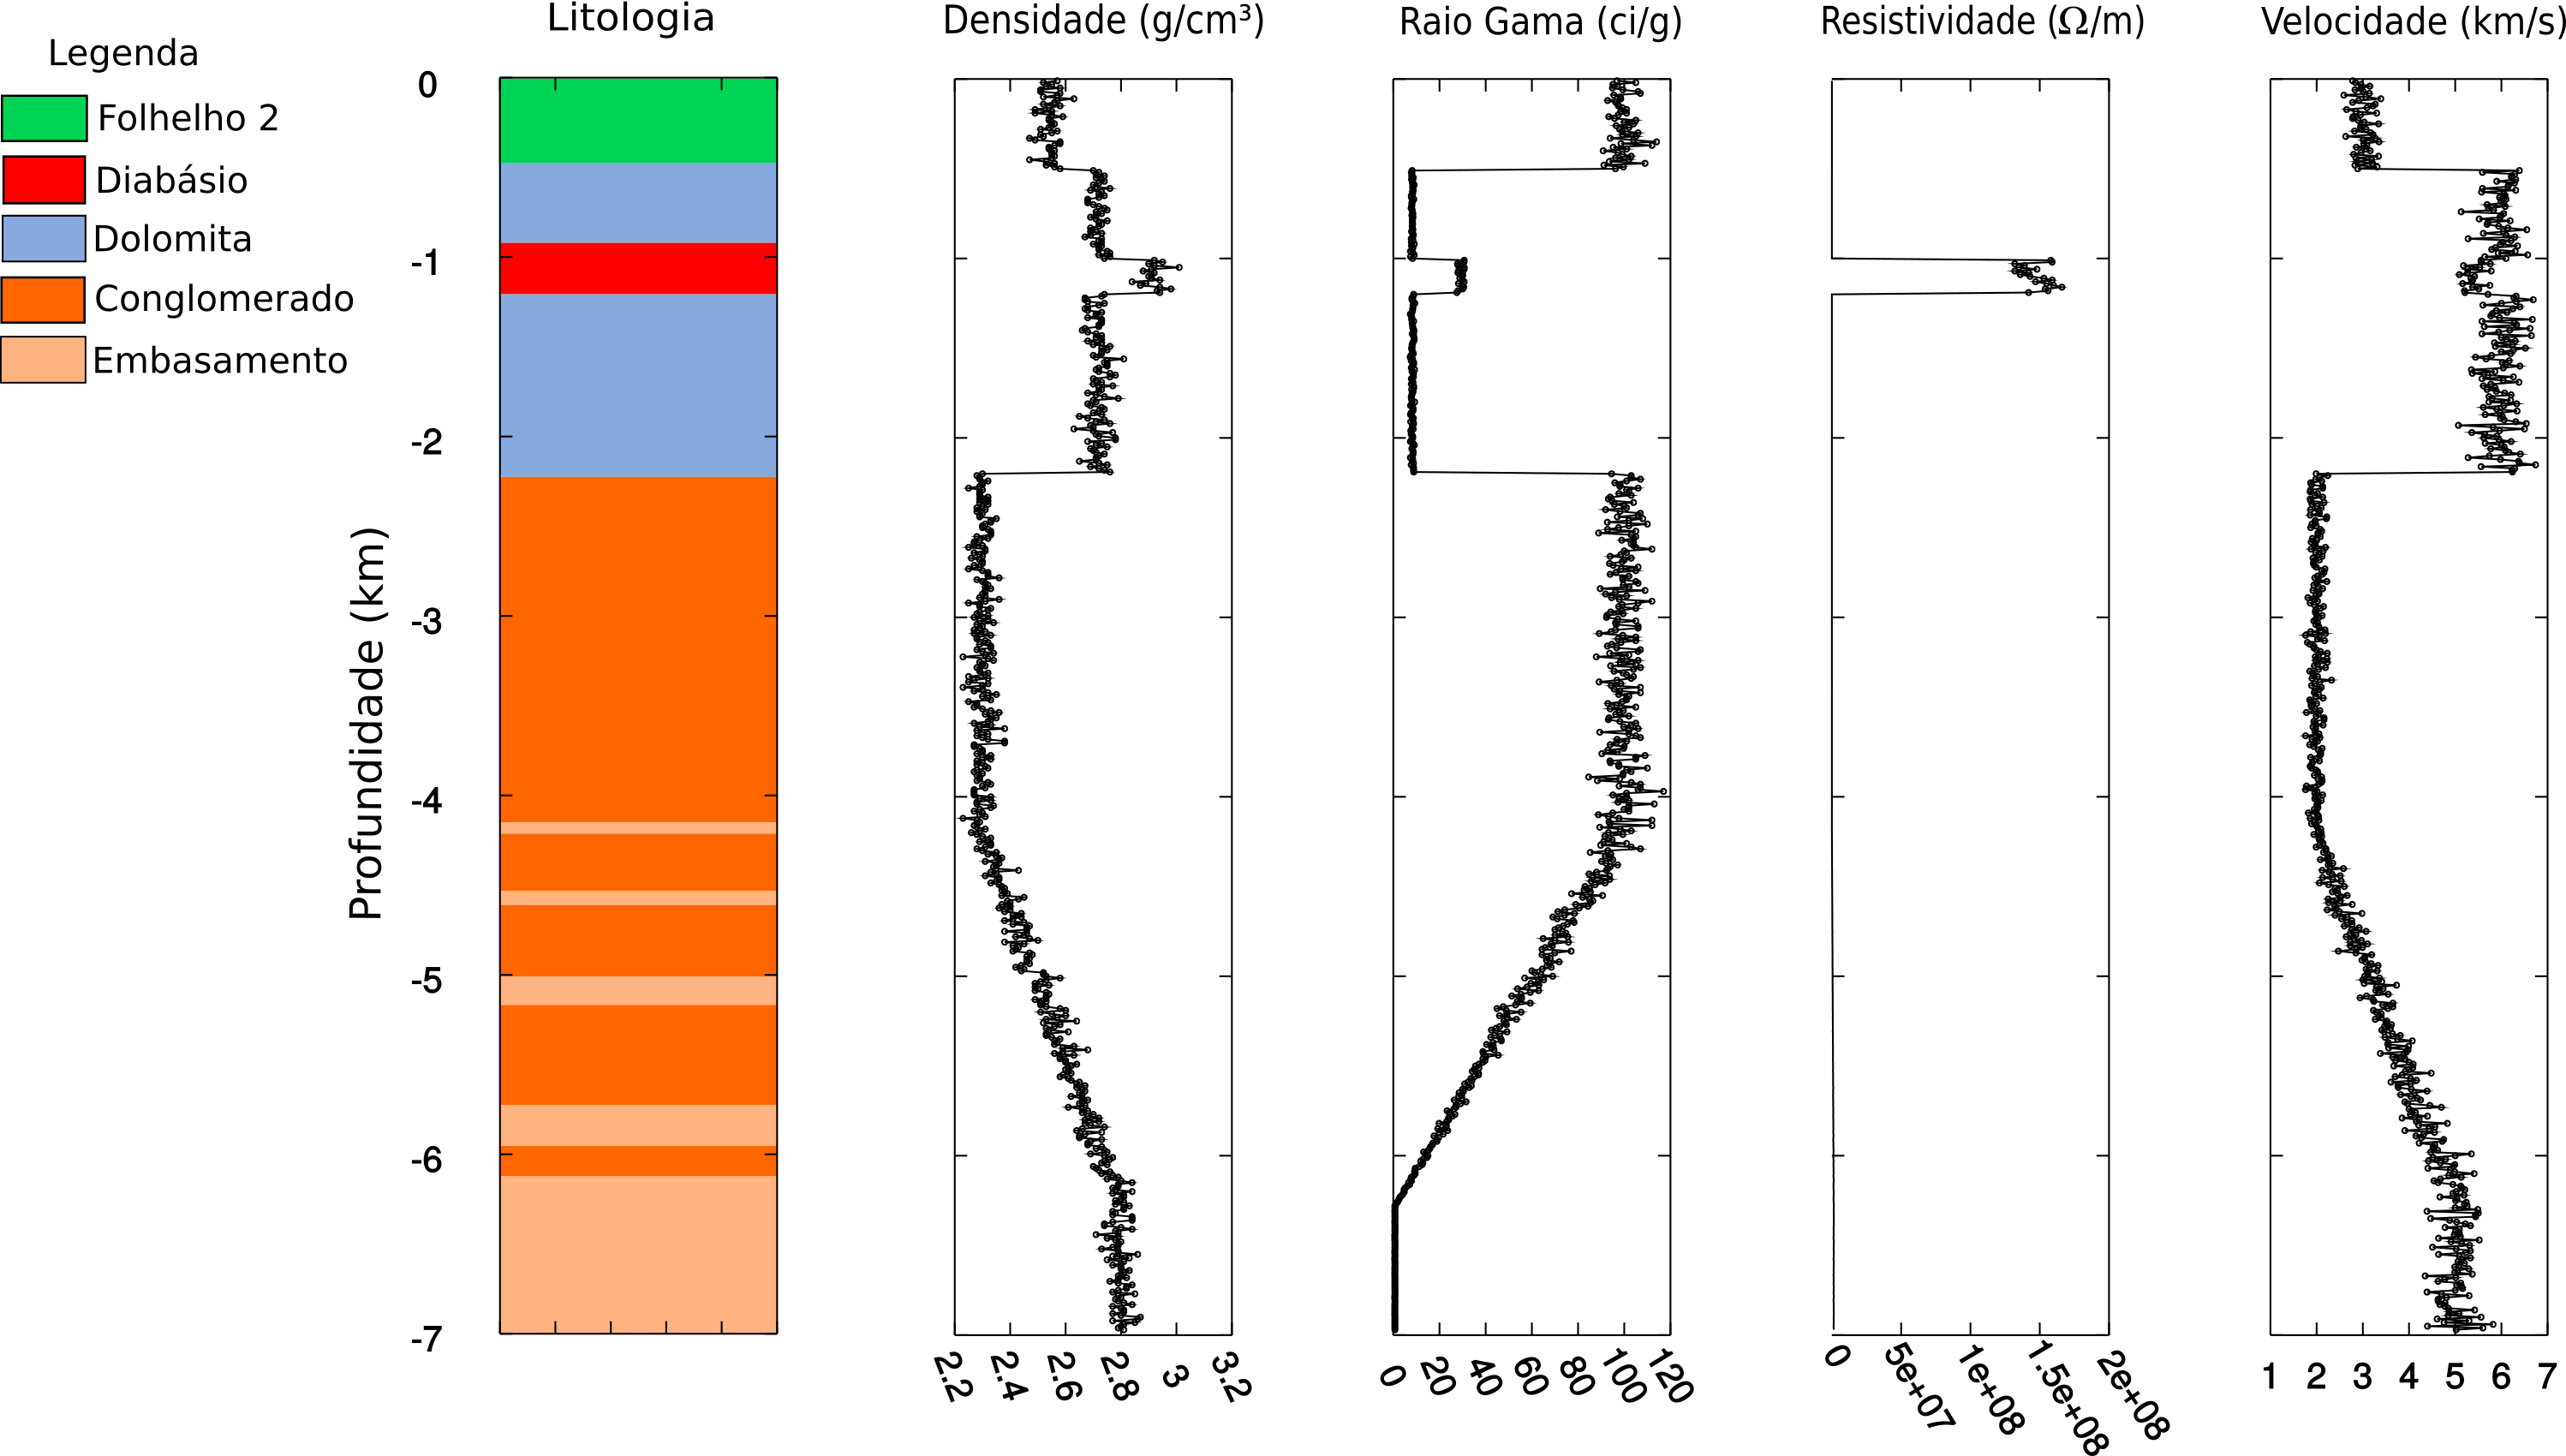
\includegraphics[scale=0.5]{Imagens/PocoT1.png}
	}
	\caption{Dado de perfilagem sintético, T1. Aonde a porcentagem de CE indica a mistura de conglomerado com embasamento}
	\label{T1}
\end{figure}

O poço C$1$\footnote{C1: Poço de classificação da rede neuronal número 1.}, Fig. \ref{C1}, possui as mesmas classes de rochas do poço T$1$. A escolha da posição dos poços quase que exclusivamente na parte SW do perfil se deu em virtude da localização do poço T$1$. Uma vez que espera-se da rede já treinada um reconhecimento das classes já estudadas. Os pacotes sedimentares apresentam espessuras de $2,8$ km de embasamento, $1,6$ km de conglomerado, $1$ km de dolomita (segundo pacote), $200$ m de diabásio, $500$ m de dolomita (primeiro pacote) e $500$ m de folhelho. 

\begin{figure}[H]
	\centering
	\setlength{\fboxsep}{8pt}
	\setlength{\fboxrule}{0.1pt}
	\fbox{
		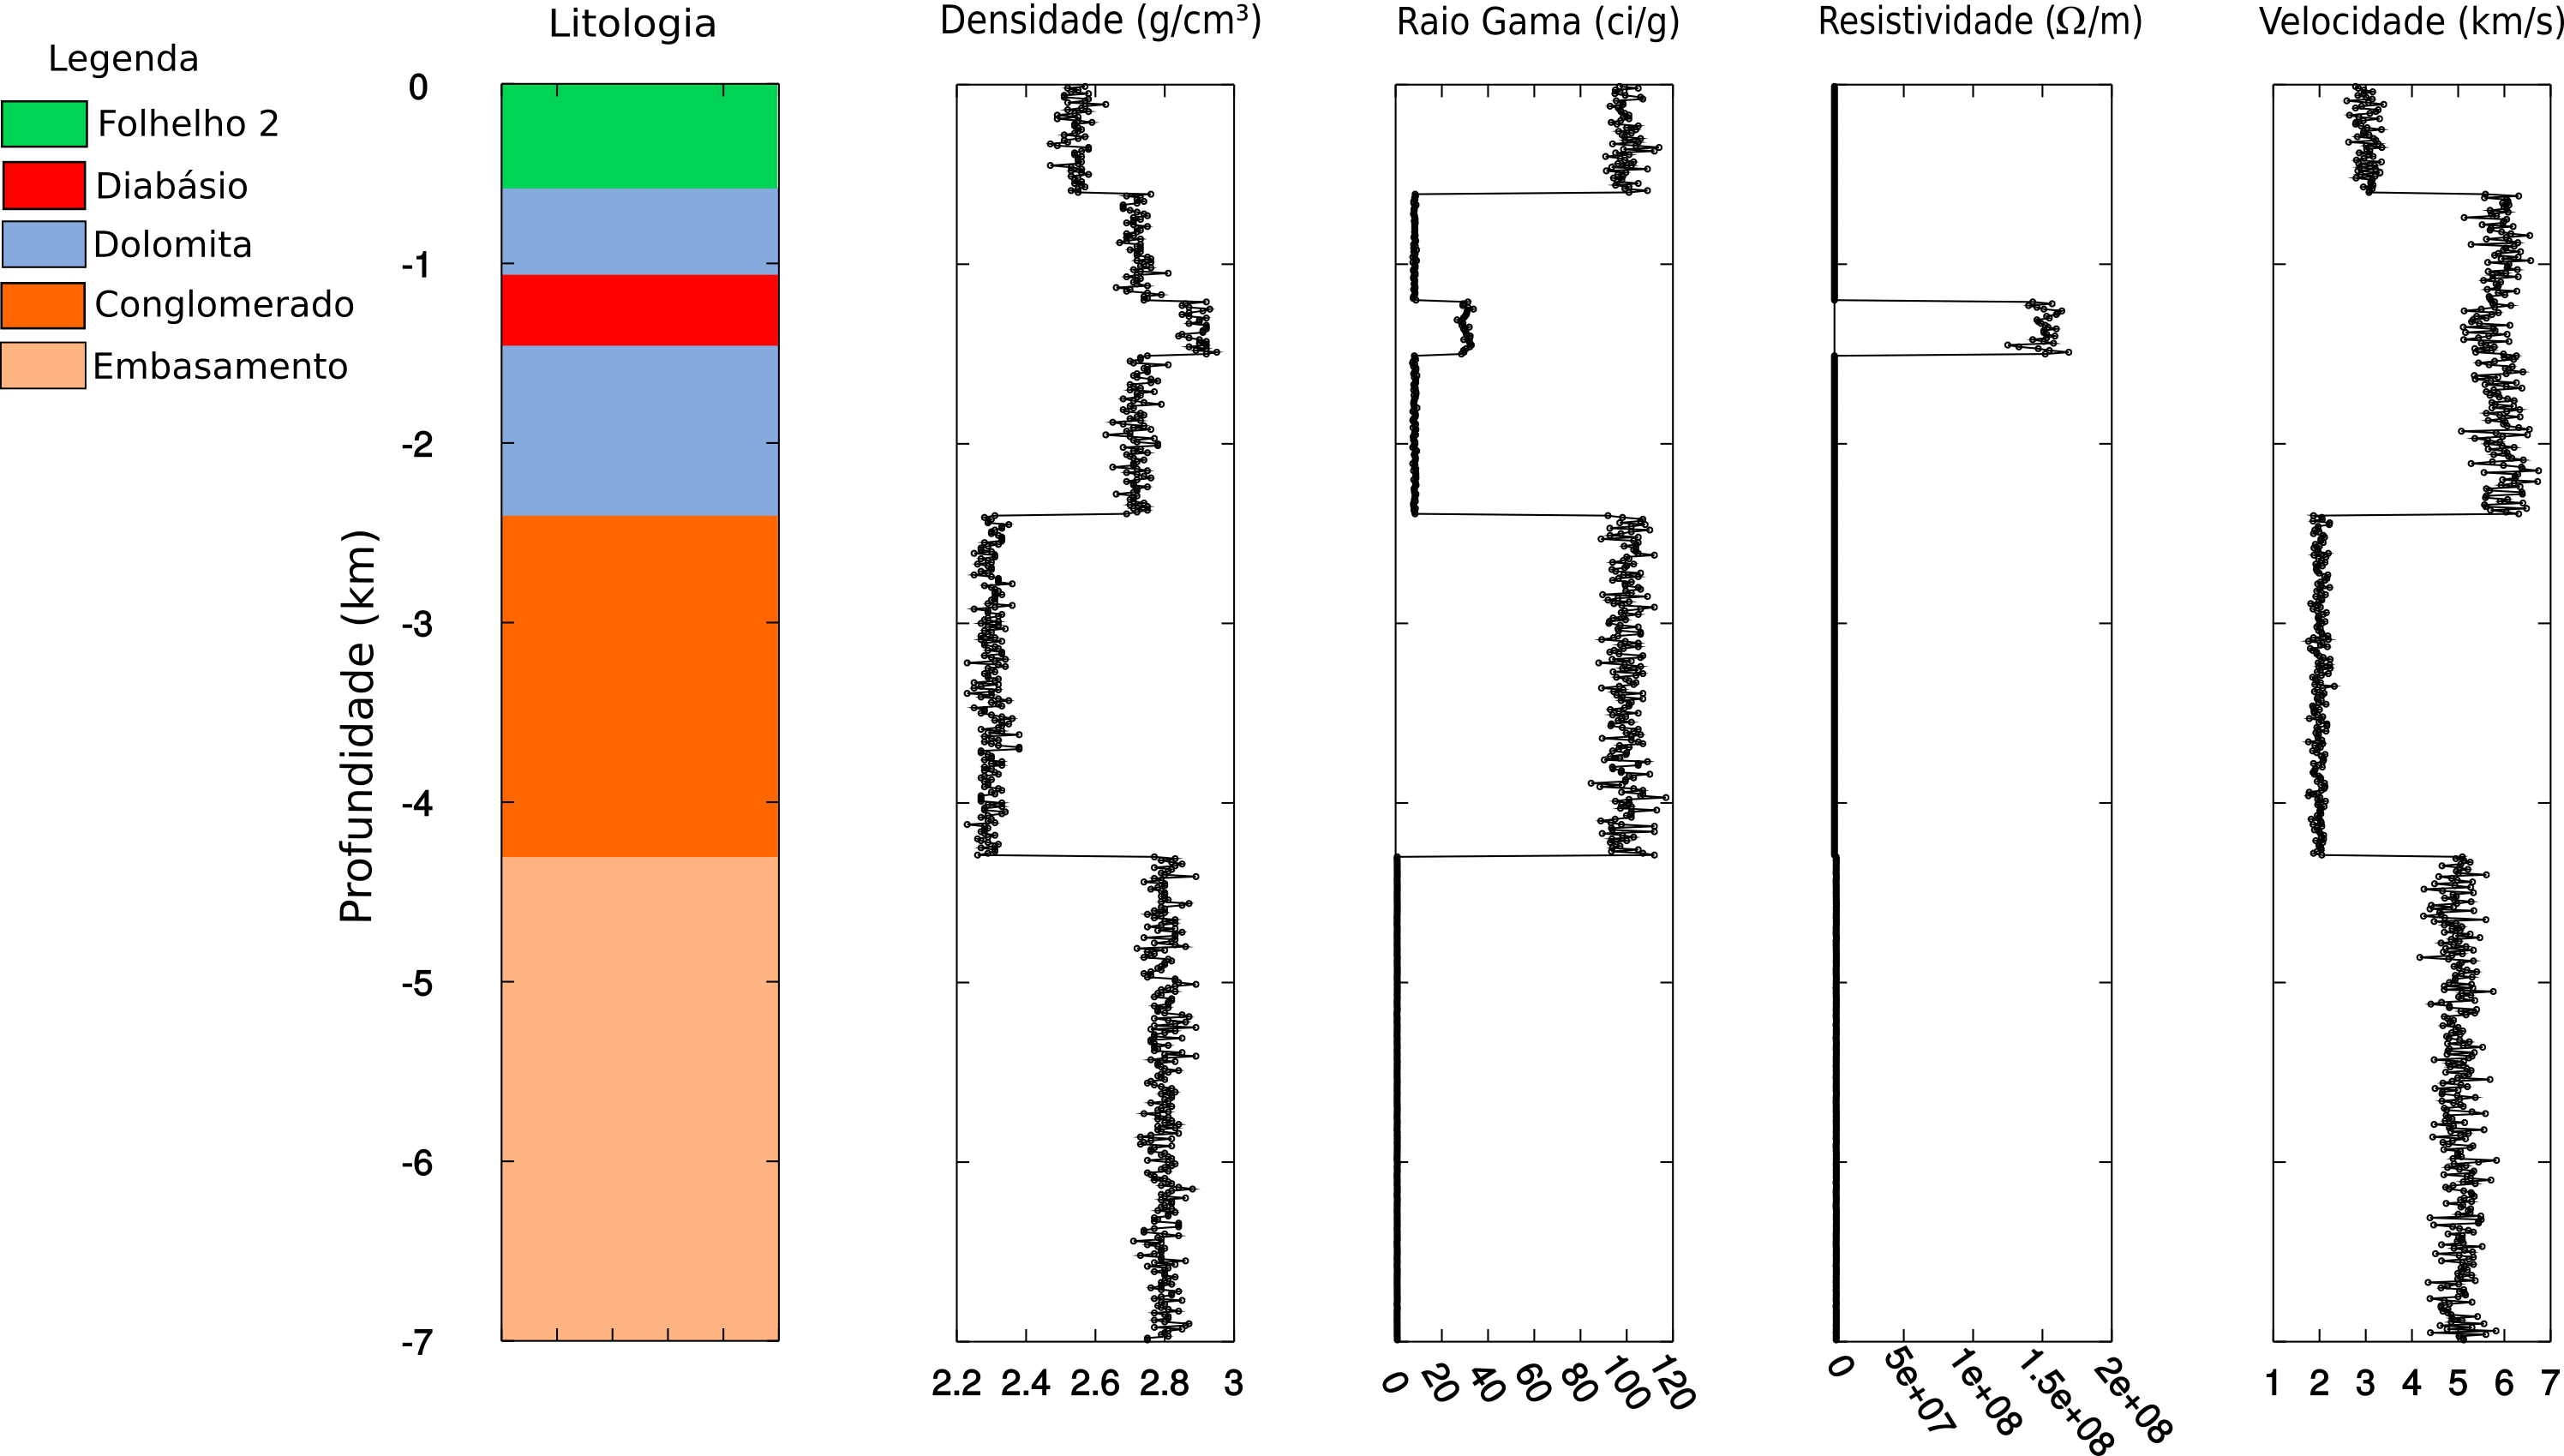
\includegraphics[scale=0.5]{Imagens/PocoC1.png}
	}
	\caption{Dado de perfilagem sintético, C1.}
	\label{C1}
\end{figure}

O poço C$2$\footnote{C2: Poço de classificação da rede neuronal número 2.}, Fig. \ref{C2}, localiza-se em um alto estrutural, e apresenta espessura de $5$ km de conglomerado. O embasamento possui uma espessura de $1,8$ km. Os pacotes de folhelho 2, dolomita (pacote superior) e diabásio $500$ m respectivamente. E o segundo pacote sedimentar de dolomita $1,6$ km.

\begin{figure}[H]
	\centering
	\setlength{\fboxsep}{8pt}
	\setlength{\fboxrule}{0.1pt}
	\fbox{
		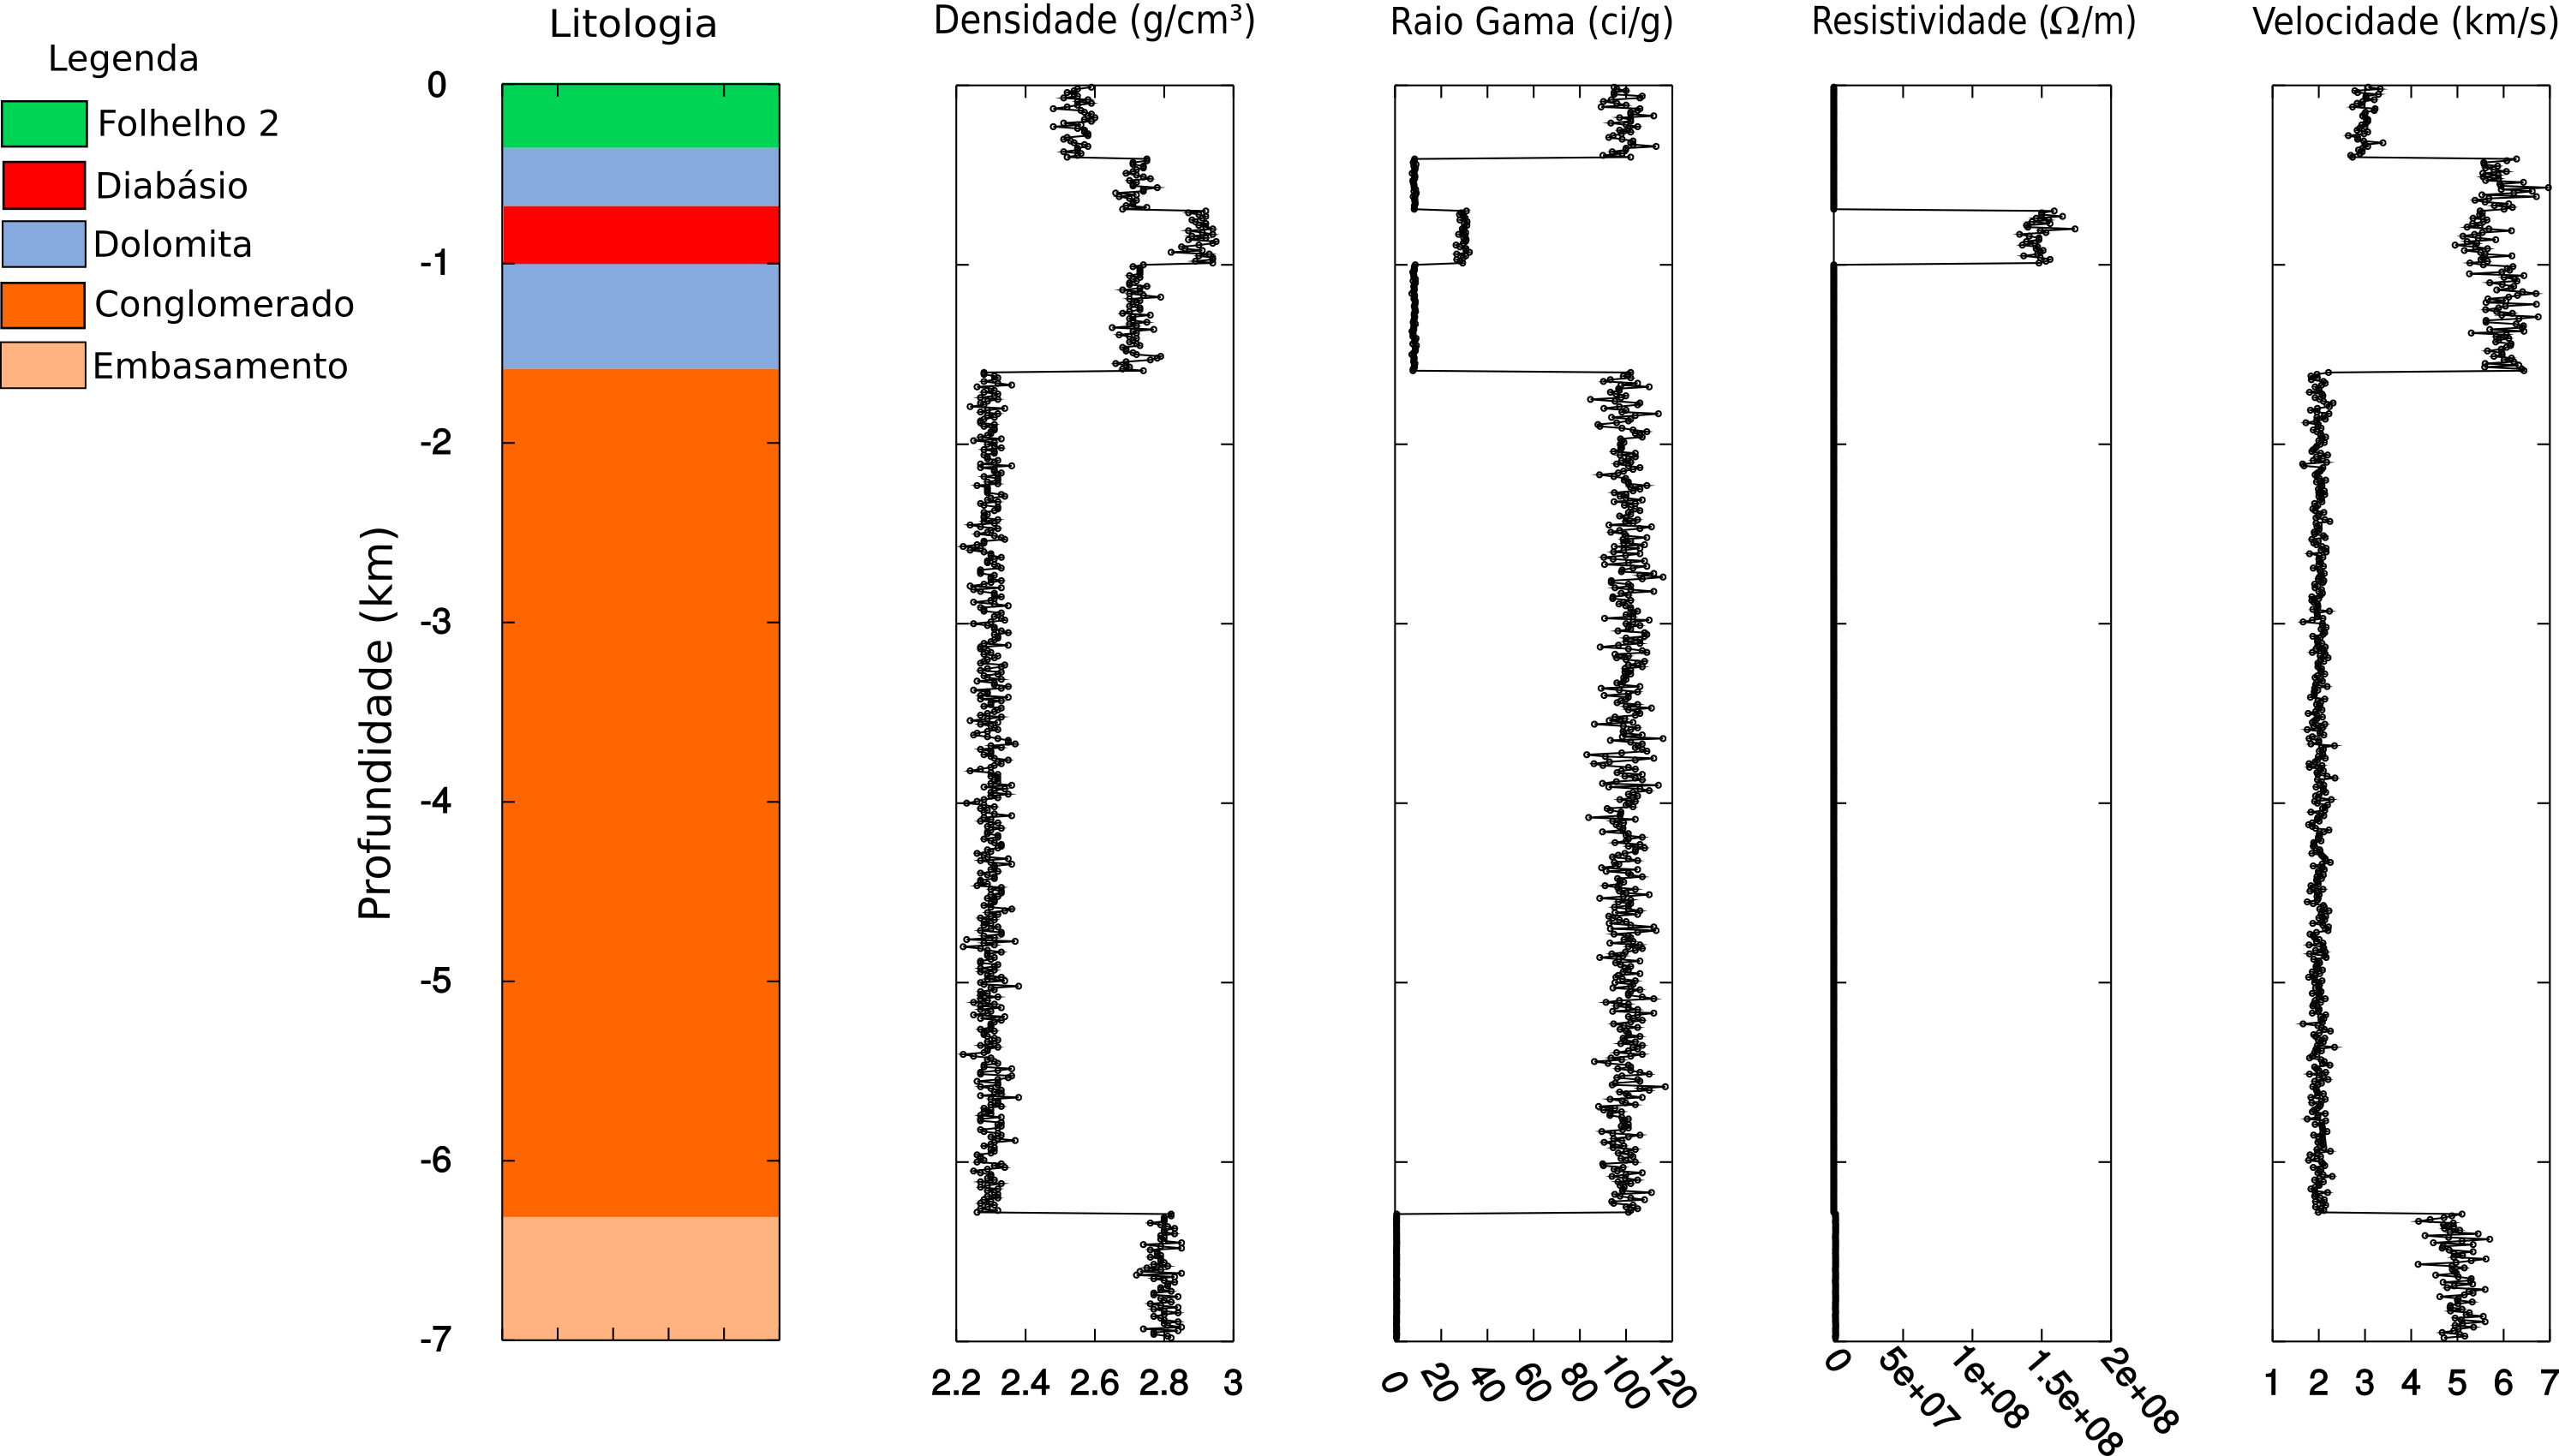
\includegraphics[scale=0.5]{Imagens/PocoC2.png}
	}
	\caption{Dado de perfilagem sintético, C2.}
	\label{C2}
\end{figure}

\section{Dado Real}

A triagem dos dados públicos contemplaram  $506$ arquivos *.dlis, $113$ arquitov *.lis, $118$ dados adicionais, $125$ perfis compostos digitalizados, $174$ poços públicos, $120$ arquivos *.agp, todos localizados na Bacia Sedimentar do Paraná. 

O conjunto de dados *.lis e *.dlis estão sendo convertidos para arquivos em formato texto, que serão posteriormente concatenados  com os arquivos *.agp afim de se obter o input da rede. Este processo ainda se encontra na fase inicial com cerca de $3\%$ concluído.

A Fig. \ref{real} mostra a localização e distribuição dos poços na Bacia do Paraná.

\begin{figure}[H]
	\centering
	\setlength{\fboxsep}{8pt}
	\setlength{\fboxrule}{0.1pt}
	\fbox{
		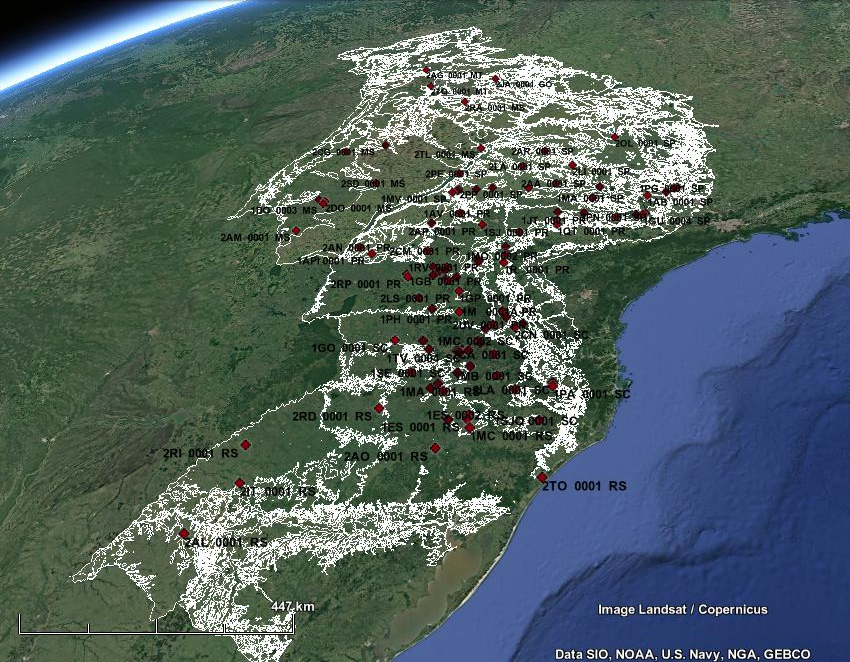
\includegraphics[scale=0.5]{Imagens/Pocos.jpg}
	}
	\caption{Localização dos poços de trabalho.}
	\label{real}
\end{figure}


